\startchapter{GPU discretization}
\label{chapter:GPUDiscretization}
In the previous chapter we presented an algorithm for fast triangle mesh extraction from \blob scene graphs. The output of that 
algorithm is a list of vertices with their associated attributes such as position, color and normal and a list of triangles that
defines the connectivity of the surface mesh. While the surface mesh is used for rasterization it can also facilitate  
collision detection and contact modelling algorithms as we will see in the following chapters.  In this chapter we propose an improved 
version of that algorithm that can take advantage of the processing capabilities of the GPU and provides real-time \blob rendering performance. 

Building on top of the results from our SIMD polygonization algorithm, in this chapter we present our work in optimizing that 
algorithm for many-core architectures such as GPU. When compared to the related work in the field, our proposed method has the following
benefits:

\begin{itemize}
 \item It is data-driven, i.e. the input to our algorithm is a dynamic \blob structure that can change 
 in every frame. This is a key advantage that can enable interactive modelling sessions in an implicit 
 framework, i.e. the result of modifications to the model can be viewed in real-time.

 \item The proposed GPU-based data-structure is compact enough to enable rendering complex \blob models 
 in the order of 60,000 nodes. (64,000 nodes only requires about 20MiB of video memory in our system).
\end{itemize}

In the following we review the related work in this domain and continue with a discussion in differences of many-core 
architectures. The data-structure and the algorithm are explained in the following sections. The chapter concludes with 
the results and analysis.



\section{Related Work}
GPU accelerated rendering techniques has been the topic of interest for the graphics community in the past two decades.
Several GPU-accelerated algorithms have been proposed for fast triangulation and rendering of iso-surfaces that are defined by
volume data-sets, algebraic surfaces and radial-basis functions. In this section we will review the most related works.

Chochl{\'i}k \etal proposed a GPU accelerated polygonization algorithm for dynamically changing implicit surfaces \cite{chochlik2012gpu}. 
Their method is based on the marching tetrahedra (MT) algorithm. The model is partitioned into cubic cells first and then each cell is 
subdivided into 6 tetrahedra to be further processed using the GPU geometry shading stage. The vertices are marked inside if their 
associated field is above zero and outside otherwise. A configuration index is computed per each tetrahedra based on the inside/outside 
vertices. The triangle mesh is produced which is shaded using the fragment shader stage. No further analysis has been made on the performance 
of their algorithm and the input models are limited to time varying simple algebraic surfaces. The used a linear interpolation root finding
method which produces low quality output. 

Buatois \etal proposed a GPU accelerated iso-surface extraction method based on MT, similar to Chochl{\'i}k \etal \cite{Buatois2006}. The 
texture memory to transfer the position and field values of the grid vertices. They presented an analysis of the performance of their algorithm
using a fluid simulation volume data-set. They reported that excessive texture fetches can be a bottleneck in the performance of their method.


Tatarchuk \etal proposed a GPU iso-surface extraction algorithm which is a hybrid of marching cubes and marching tetrahedra \cite{Tatarchuk2007}. 
They start by voxelizing an implicit grid into discrete cube cells and then convert that to a tetrahedral representation. They implemented an MT 
algorithm on geometry shader stage of DirectX10 API. For root finding method they fitted a parabola along the intersecting edges and evaluated a 
quadratic equation which produces a better approximation. They tested their system using the visible human volume data-set. Their method
is limited to static volume datasets and is not usable in a data-driven setting where the topology of the underlying model changes. 

With modern hardware and fast GPUs, ray tracing of implicit surfaces is the subject of much research. Knoll \etal \cite{Knoll2009} presented 
CPU and GPU algorithms that can achieve interactive visualization for common algebraic surfaces. The surfaces used in by Knoll \etal are not 
arbitrary implicit models but surfaces generated using traditional kernels or functions. Similar surfaces are presented by Singh and Narayanan
for real-time ray tracing of implicit surfaces using the GPU \cite{singh2010real}. 


Kipfer and Westermann \cite{Kipfer2005} accelerated rendering of implicit surfaces by avoiding redundant computation of edge surface intersections. 
Our method also employs this feature to reduce the overhead. They also use features of the GPU to reformulate the iso-surface identification and reduces 
numerical computations and memory access operations. They used a span-space data-structure to avoid processing non surface intersecting elements.

Kanai \etal \cite{Kanai2006a} proposed a rendering method for sparse low-degree implicit surfaces (SLIM) using ray casting approach. The ray and IS intersection
test has been carried out on the fragment processing stage. They employed level of detail rendering and view frustum culling to speedup the rendering. 
The coefficients for the IS are passed in using textures. They reported high quality and interactive rates for several models. The large number of processed
fragments is the bottleneck in this process and models with lower number of nodes could be rendered slower than more complex models that cover less fragments.
Although Kanai \etal's work is data-driven but the increasing cost of fragment processing is the main bottleneck in their system. Also since they are not
producing any mesh the computations will be lost after rendering.



%Another requirement for the tetrahedral mesh generation is that the triangular surface mesh should be the boundary surface of the tetrahedral mesh. This is needed since 
%after applying the displacements to the volumetric tetrahedral elements the surface vertices should be displaced as well.
\section{Many-cores architectures}
Shrinking of CMOS circuitry has allowed distances between transistors to scale fairly consistently for an extended period of time. The shrinking 
of distances and reduction in size of capacitors allowed hardware architects to clock circuits at a higher rate. This led to Gordon Moore's
famous self fulfilling prophecy about transistor density and its misinterpretations into the realm of execution frequency and overall performance.

Certainly, increasing frequency allowed the performance of nonparallel code to increase consistently during that time, such that it became an 
expectation for software developers until the early 21st century. During the past decade, it has become obvious the continued scaling of clock 
frequencies of CPUs is not practical, largely due to power and heat dissipation constraints. The reason for this is that power consumption is 
dependent on frequency in a nonlinear manner \cite{gaster2012heterogeneous}. As a second problem, increasing clock frequency on-chip requires 
either increasing off-chip memory bandwidth to provide data fast enough to not stall the linear workload running through the processor or increasing
the amount of caching in the system. 

Due to those reasons the computational hardware available in high-performance workstations shifted from increasingly efficient but complex sequential 
computational units, to smaller units which are not faster than previous generations but the cores are duplicated to be able to execute more threads 
in parallel. This new trend in design can be found in modern CPUs and recent Graphics Processing Units (GPUs). The latest generation of GPUs contains 
hundreds of computation units (4096 in AMD Radeon 7990, 2496 in NVIDIA Tesla K20. For a brief discussion on how to count GPU cores refer to \cite{Fatahalian2008})

This radical architectural change has important consequences on the type of algorithms which are applicable in interactive simulations. In terms of 
programming, general purpose computations on GPUs initially required the use of graphics oriented libraries. The two major GPU vendors released general
programming APIs, CUDA \cite{Nickolls2008} and CTM \cite{peercy2006performance} which provide direct access to the underlying parallel processors of the
GPU, as well as full instruction sets, such as double precision computations and write operations at arbitrary locations. OpenCL which is a multi-vendor
standard was released in 2009, with a programming model very similar to CUDA \cite{gaster2012heterogeneous}. The presented algorithms in this chapter
have been implemented in OpenCL. 

In OpenCL and CUDA threads may access data from multiple memory spaces during their execution \cite{Nickolls2008}. Each thread has a 
private \textit{local} memory. OpenCL uses this memory for thread-private variables that do not fit in the thread's registers, as well 
as for stack frames and register spilling. Each thread block has a shared memory visible to all threads of the block that has the same 
lifetime as the block. Finally, all threads have access to the same \textit{global} memory. 

Programs declare variables in shared and global memory with the \texttt{\_\_local} and \texttt{\_\_global} type qualifiers. On a Tesla-architecture 
GPU, these memory spaces correspond to physically separate memories: per-block shared memory is a low-latency on-chip RAM, while global memory 
resides in the fast DRAM on the graphics board. 

Shared memory is expected to be a low-latency memory near each processor, much like an L1 cache. It can therefore, provide for high-performance 
communication and data sharing among the threads of a thread block. Since it has the same lifetime as its corresponding thread block, kernel 
code will typically initialize data in shared variables, compute using shared variables, and copy shared memory results to global memory. 
Thread blocks of sequentially dependent grids communicate via global memory, using it to read input and write results. 

%Register spilling can increase the number of instructions required to generate prefetch addresses. Ideally only a single instruction would be needed for each prefetch,
% i.e. the prefetch instruction itself. In some cases, as many as 20 extra instructions were added for each prefetch. 
Register spilling occurs whenever the register allocator runs out of registers, and therefore must ``spill'' values by saving and restoring them from memory. Once 
register spilling occurs, the instruction count within a loop body can increase dramatically. 
 
A potential cause of register spilling is the loop unrolling. Once a loop is unrolled, the compiler can optimize across the several replicated copies of the loop 
body. In most cases this allows the compiler to reduce the overall instruction count for the following reasons:
 
 \begin{enumerate}
  \item branch instructions can be eliminated between unrolled iterations
  \item it is more likely that ``hazard'' slots after multi-cycle operations can be filled with independent instructions. 
  \item register allocations can be optimized across the unrolled iterations, possibly eliminating loads and stores.
 \end{enumerate}

On the other hand the potential downside of the loop unrolling is creating too many intermediate values for the register allocator to handle, thus resulting in 
register spilling. One way for the compiler to avoid those register-spilling problems is to perform loop unrolling with a greater awareness of its effect on register 
pressure. 

\section{Data Structures}
\label{sec:datastructure}
The \blob linearization step introduced in (section \ref{sec:linearization}) is modified to create a compact representation of the input model in our 
GPU polygonization algorithm. 

All the structures are aligned at 16 bytes (four floating points) memory addresses (This is similar to the texture 
accessing techniques in graphical shader programming languages such as (GLSL or Cg) where four floats represent the 
RGBA values of a texel accordingly.) If a primitive node has an associated transformation node with a non-identity 
transformation matrix, that matrix will be stored in the primitive matrices section of the input structure and an 
associated identifier (id) will be provided to the primitive. The default id is 0 which points to an identity transformation 
matrix. The inverse of the primitive matrix is computed and the first three rows of it will be stored for further field 
computations. To transform the axis-aligned bounding boxes of the primitives the full forward transformation matrix will 
be stored in the box matrices section of the structure and it can be accessed using the same id provided for the primitive matrix.
Figure (\ref{fig:datastructure}) depicts this pointerless representation in details.

\begin{figure}[H]
  \centering
  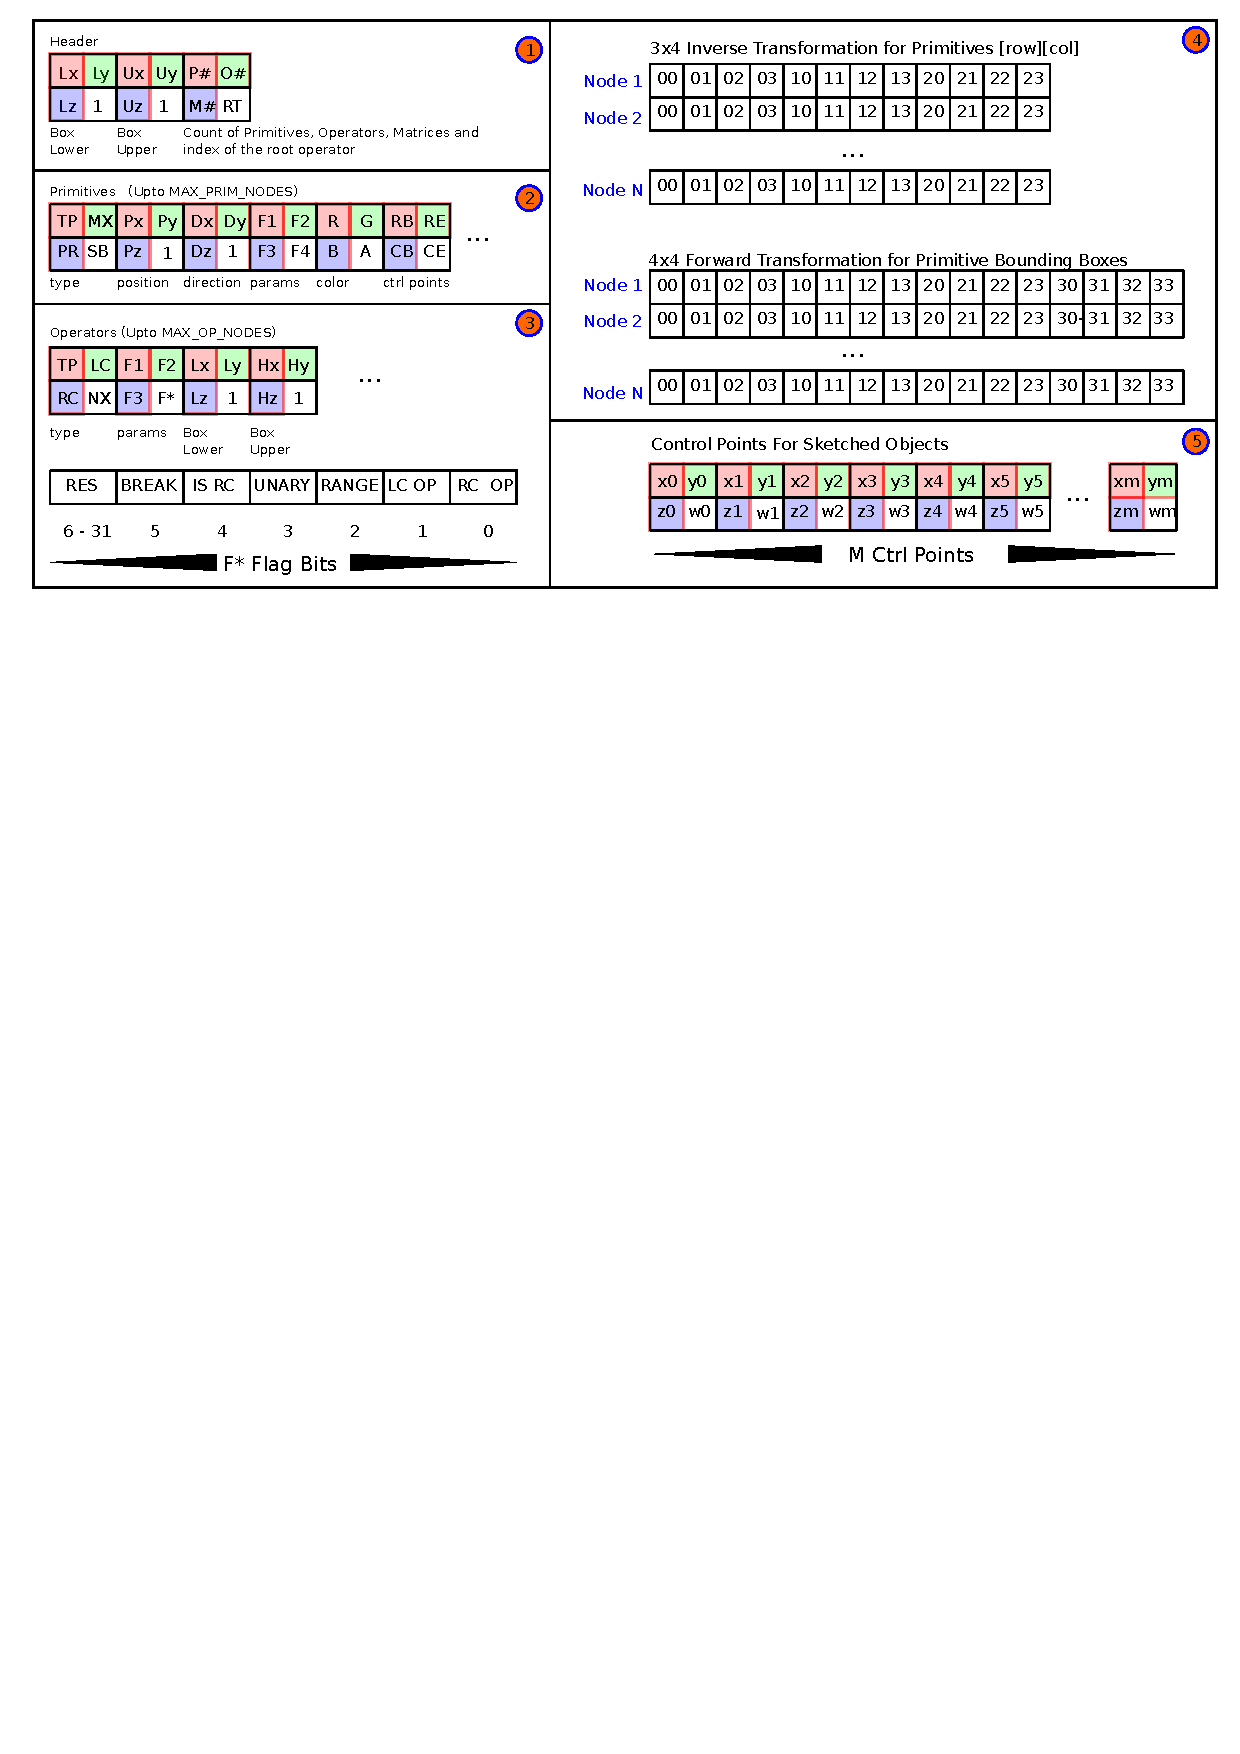
\includegraphics[width=1.0\linewidth]{figures/gpupoly/lineartree.pdf}
  \caption{\label{fig:datastructure}
  {The compact \blob scenegraph representation for GPU polygonization and tetrahedralization algorithms. The structure is 
  aligned at 16 bytes (4 floats). 1- The header. 2- Skeletal implicit primitives. 3- Operators. 4- Affine transformation 
  nodes. 5- Control points for sketched objects. Refer to section \ref{sec:datastructure} for details.}
}
\end{figure}

Each input data-structure is numbered in figure (\ref{fig:datastructure}) for further reference. We review the details in the following:
\begin{enumerate}
 \item The header section defines the lower and upper corner of the axis-aligned bounding box enclosing the entire model, 
 i.e. the convex hull of the input \blob. The header also contains the count of primitives, operators and the transformation 
 nodes. The id associated with the root operator of the tree is also defined in the header.
 
 \item The definition of each primitive is encoded in 6 texels. The $TP$ field in the first texel numerically encodes the 
 type of skeletal primitive. The other three fields in this texel are $MX$, $PR$ and $SB$ that link this primitive to its inverse 
 transformation matrix, the parent and the sibling elements respectively. The following texels define the position, 
 direction, skeleton-specific parameters and the color of the primitive. For the primitives that are 
 computed from sketched control points (e.g. the thin-plate spline primitives \cite{Turk1999, Grasberger}) the indices to the 
 associated first and last control points are stored in the last texel.

 \item A \blob operator is defined in 4 texels. The type of the operator is defined first in the $TP$ field. 
 The following fields define the left and right children, in case all the children are primitives and their indices are in 
 consecutive order (e.g. a range); $LC$ and $RC$ are the indices to the first and last children respectively. This situation 
 can happen if an operator is applied to a list of consecutive primitives, e.g. a global union operator.  The $NX$ 
 field is related to our stackless \blob traversal algorithm which is explained in the following sections and defines the next 
 operator node in the \blob traversal route. The operator-specific parameters and its axis-aligned bounding box are stored next. 
 The $F^*$ flag provides more control over the operator and the definition of its bits can be found at the bottom of figure
 \ref{fig:datastructure}. Bits 1 and 0 are set in case the left child or the right child of the current node are operators as well. Bit 2 is 
 set if the $LC$ and $RC$ indices are actually defining a range of skeletal primitives as explained earlier. In this case the 
 first two fields will be set to zero. If the unary flag is set then the operator has only one child which stored in the $LC$ field.  
 Bit 4 is set when the current operator appears as a right node for its parent. Bit 5 is the break route flag and is discussed further 
 in our stackless \blob routing algorithm. The rest of the bits are reserved for future use. 
 
 
 \item As mentioned above the inverse of the transformation matrices are computed and the first three rows are stored in our input 
 structure for field computation purposes. The elements are depicted in the format of [row][column]. The forward transformation is 
 stored as a 4x4 matrix in a separate input structure for performance reasons. 
 
 \item The control points associated with the sketched primitives are all stored in this section. Each control point is defined with 
 their XYZ coordinate and an associated weight value. 
\end{enumerate}

\section{Memory foot prints}\label{sec:memory}
After analyzing the performance of our OpenCL kernels, register spilling often found to be the major cause for many latencies. Resorting to shared memory spaces, reducing 
number of intermediate variable in field-evaluation kernels and avoiding loop unrolling in some cases helped to optimize the performance. Upon every
change in the input \blob the scene-graph is compacted and transferred from main memory to the GPU. Currently the maximum number of nodes is set at 64K which covers
all of the complex cases we modelled for this thesis. However, for larger \blob models  we can easily increase this amount to support them. The memory footprint of 
our current \blob representation is summarized in table \ref{table:memfootprint}. Each row in the table represents a \blob with a specific number of nodes.
Starting from the simplest \blob with only one node (e.g. a sphere primitive) to the most complex \blob with one million nodes. The middle columns in the 
table are the break down of the required memory size per each component in the compacted \blob data structure.

\begin{table}[H]
\begin{center}
	 \caption{\label{table:memfootprint}
  {Memory footprint of the input \blob in our GPU polygonization algorithm in bytes. The entire \blob for a model with 64K nodes (primitives and operators) 
  takes about 20MB in our current system.}
}
  \begin{tabular}{ | c | c | c | c | c | c | c | c |}
    \hline    
    Nodes & Header & Primitives & Operators & Prim Mtx & Box Mtx & Ctrl Points & Total \\ \hline \hline
    1 & 48 & 96/Prim & 64/Op & 48/Prim & 64/Prim & 16/Point & 320 \\ \hline
    1K & 48K & 96K & 64K & 48K & 64K & 16K & 320K \\ \hline
    64K & 3072K & 6144K & 4096K & 3072K & 4096K & 1024K & 20M \\ \hline
    1M & 48M & 96M & 64M & 48M & 64M & 16M & 320M \\ 
    \hline
  	\end{tabular}
\end{center}
\end{table}


\section{Stackless \blob traversal}
\label{sec:stackless}
As shown in figure \ref{fig:TowerSNBTimeBreakDown} the major bottleneck of the algorithm presented in chapter 
\ref{chapter:cpuPoly} is the surface extraction process. The expensive operations in that 
stage is the computation of normals and colors which require extra field evaluations and hence performance degradation. 

In this section we describe our novel stackless \blob traversal algorithm. 
Without a stack to be maintained the \blob traversal incurs less memory footprint. When dealing with small 
local memory available per each thread on the GPU this reduction in memory usage improves the performance of the 
running kernels significantly.

In high performance rendering algorithms the use of hierarchical spatial data structures for acceleration reasons 
is common. Vising nodes in such structures requires stack-based traversal algorithms. Unfortunately, even the latest 
GPU architectures are poorly suited for implementing such algorithms. 

A complex \blob scene-graph data structure may contain thousands of primitives and operators which can lead to deep tree structures. 
In the original stack-based traversal algorithm, the fieldvalue evaluation process has two stages: A ``down traversal'' followed by an ``up traversal''. 
During the down traversal stage all operators starting from the root node are visited and pushed onto an operators stack until a leaf node (primitive) 
is reached at which point the field due to the primitive is computed and pushed onto a separate fields stack and the next 
stage which is the up traversal begins.

During the up traversal stage the operators are popped out of the stack and per each child an associated field is popped from the fields stack for the 
operator to combine them in its own specific way. The resulting field is again pushed back on the fields stack.  This process continues until the 
operators stack get emptied and the final fieldvalue due to the root node is computed and returned.

Performing many push and pop operations limit the performance of the traversal process. The other issue relates to the 
inherently dynamic storage requirement for the stack itself. Although, creating a fixed-size stack is possible but since the stack size is a function of
the count of nodes in the input \blob, this will ultimately limit the maximum number of nodes in a complex scene. If $N$ is the maximum number of nodes 
(primitives plus operators) allowed in a \blob model then the minimum number of elements to be stored in the stack during the traversal process 
is given by: $M=\log(N)$ or the depth of the binary tree created by $N$ nodes. Recalling from section \ref{sec:memory} there is a limited amount of
local memory available per each thread executing on the GPU. Keeping the stack in the shared memory will also complicate the implementation and
the access patterns from other threads in the current thread block and may impact the performance. Needless to say that implementing a stack in the global 
video memory will require very expensive memory transfers and is not an option for a real-time rendering algorithm. 


Our algorithm is based on the neighbor cell-links concept in the stackless traversal of spatial subdivision trees 
which is first introduced by Samet \etal \cite{Samet1984,Samet1990}. Using a similar technique Popov \etal presented 
a stackless KD-Tree Traversal for high performance GPU ray tracing algorithm \cite{Popov2007}. 

%Although the \blob traversal algorithm presented here is somewhat different in my approach, a similar idea was put forward 
%by my fellow student, Herbert Grasberger, and submitted for publication. The details to be found in his thesis \cite{Grasberger2015}. 
%The following \blob traversal stage was developed independently inspired by his draft publication.

The algorithm is divided into two stages. A preprocessing stage to compute a traversal route for the entire 
\blob and the GPU-based stackless traversal stage to compute the field-value due to a given point in space. 
The following will describe these two stages in greater details.


\begin{figure}[H]
  \centering
  % the following command controls the width of the embedded PS file
  % (relative to the width of the current column)
  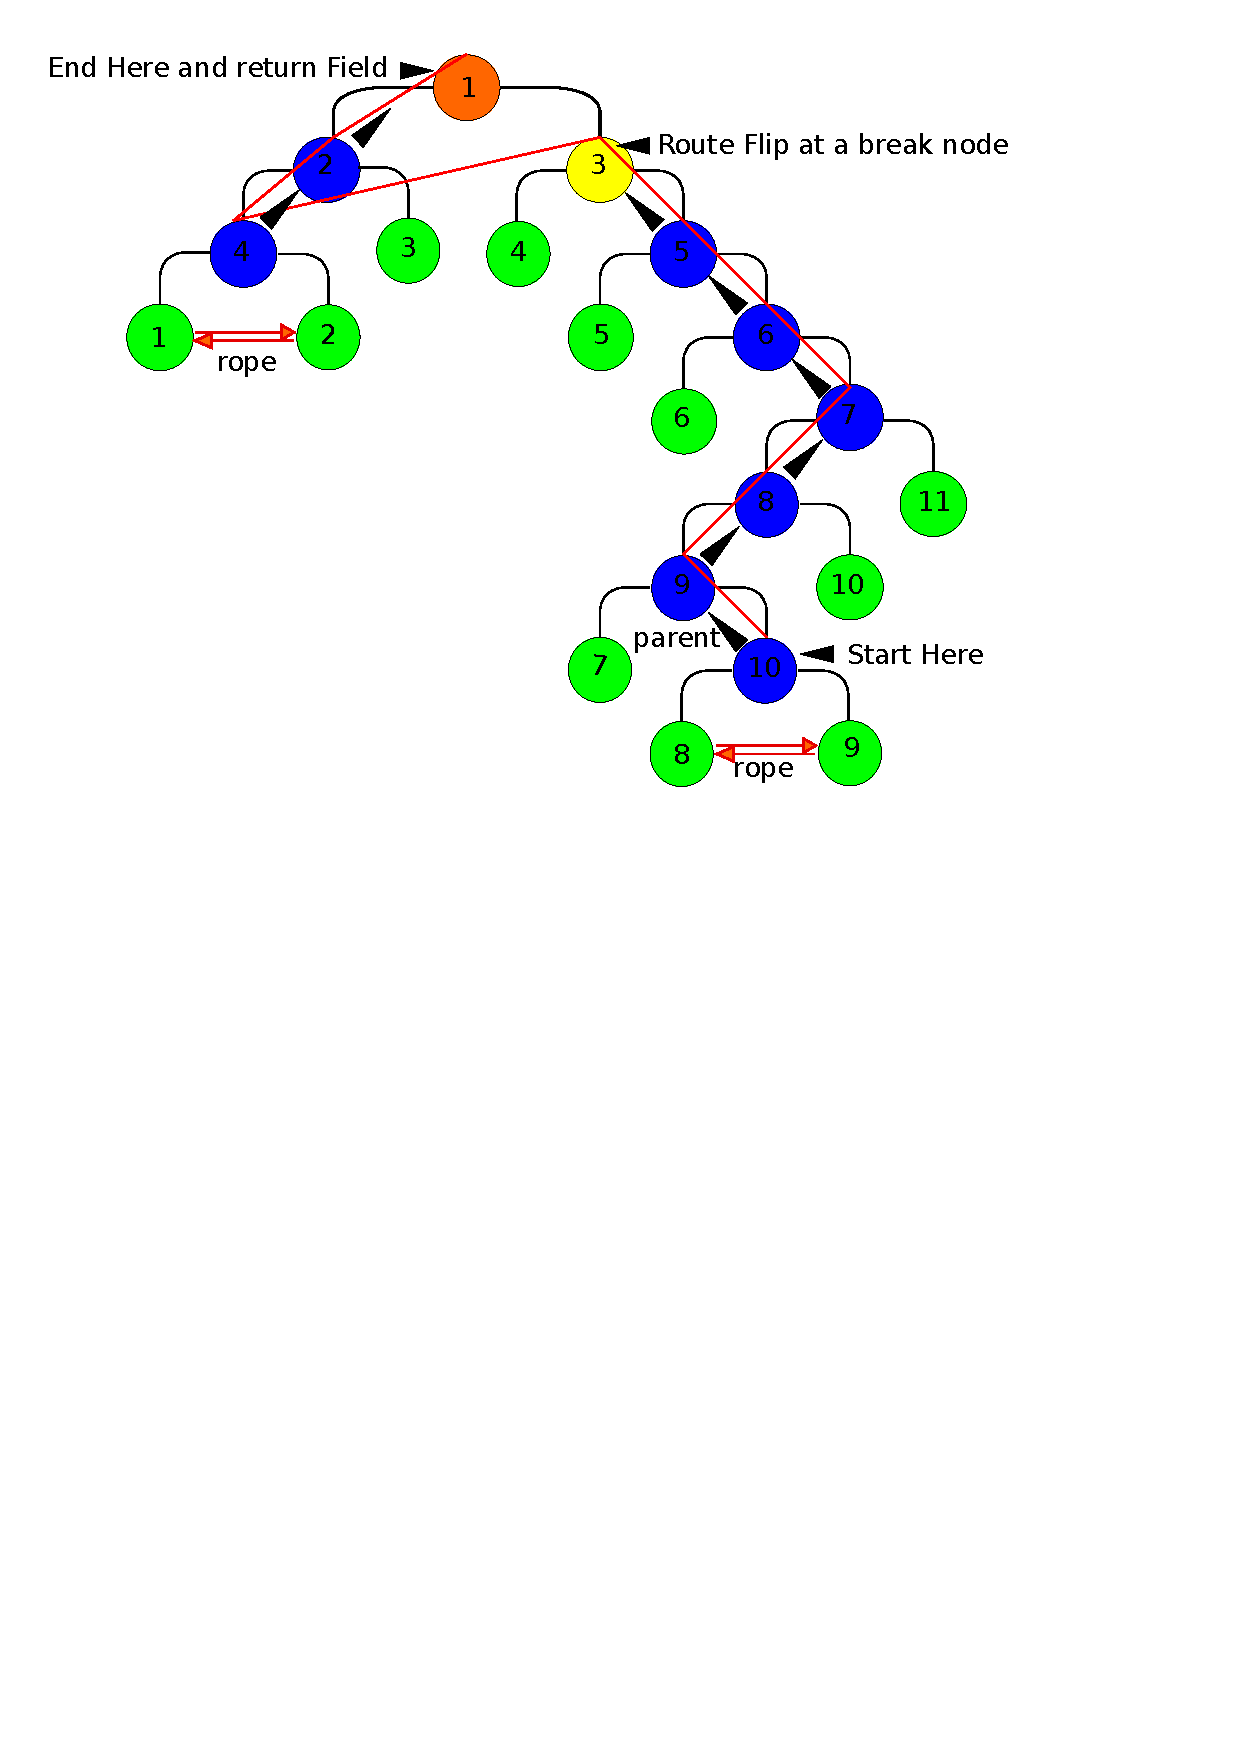
\includegraphics[width=1.0\linewidth]{figures/gpupoly/stackless.pdf}
  \caption{\label{fig:stackless}
  {Stackless \blob traversal algorithm performs faster on deep tree traversals. The route is computed once and encoded into the tree upon transferring the input 
  data structures to the GPU.}
}
\end{figure}

\subsubsection{Encoding traversal route}
The first stage in our algorithm is to compute a route to visit all nodes in the \blob 
and finally encode that route in the GPU input data-structure. This process is performed only once and is not a 
bottleneck in the system. The one-time fixed cost paid for this stage on the CPU is regained 
when many fieldvalue evaluations are performed in parallel on the GPU without the extra cost 
associated with the stack storage.

To compute the route the following steps are performed on the CPU side as a preprocessing stage: 

Using the naive \blob traversal algorithm the nodes are visited from root to leaves. Two stacks are maintained in this process, an
operators stack $S1$ and a \text{break} nodes stack $S2$. The latter is defined in the following:

\begin{enumerate}
 \item If one of the children is an operator $A$ and the other is a primitive $B$. The parent for $A$ is set 
 to the current node and then it is pushed onto $S1$.
 
 \item If both children are operators. The right child is set as a \textit{break} node and is pushed on to $S2$. 
 The route at break nodes is flipped to the left branch of the tree, see figure \ref{fig:stackless}. 
 
 \item If the two children are both primitives: First the root of the \blob is set to the current node if it has not been set before.
  (Refer to the \blob header format in figure \ref{fig:datastructure} for the location of the root field shown as $RT$.) 
  A rope is created between the two primitives, linking the two nodes and a break node $B$ is popped from $S2$. 
  The next node for $B$ is set to the current node.
 
  
 \item This process is continued until $S1$ is emptied.
\end{enumerate}


%add an algorithm listing for this

%describe what happens on the GPU as well

\subsubsection{Up-sweep traversal on the GPU}
Figure \ref{fig:stackless}, shows the final route for a sample \blob. The benefits of this type of routing encoded into the tree
is that there is no need for storing a deep stack to store the intermediate operators. Using this new approach the tree is now only evaluated 
from bottom to top. 

The \blob root node $RT$ marks the starting point of the traversal. This field is stored in the header section of the 
data structure as illustrated in figure \ref{fig:datastructure}. Using the new traversal route this field is set to
the operator node 10 for the example \blob shown in figure \ref{fig:stackless}. 

In case of an operator where all its children are primitives, the field due to each child is computed before the operator evaluation. 
The computed field is stored in the global field variable $F1$ and using the link to the next node provided in the structure ($NX$) 
the evaluation continues to the next operator in the tree at an upper level (up-sweep). When evaluating an operator with one primitive
child then the field due to the primitive child is computed before applying the current operator to $F1$ and performing the up-sweep (nodes 5 to 9 in 
figure \ref{fig:stackless}).

When visiting a break node the field is computed as usual but this time it is stored in the special variable $F2$, instead. 
In addition at a break node, the $NX$ field in the structure points to a non-parent operator (operator 4 for break node 3 in the example).

The process continues until the first node in the tree is evaluated at which the $F1$ and $F2$ values store the children fields for 
their parent. The $NX$ field associated with the first node points to itself which marks the end of the traversal process.


\section{GPU Surface Extraction Algorithm}
\label{sec:surfextraction}
In this section we present our GPU polygonization algorithm which is based on our novel field value evaluation technique described
in the previous section. Since the following steps are implemented using OpenCL on the GPU we will use the term \textit{kernel} which 
is a single thread of execution on the GPU. Please refer to section \ref{sec:memory} for a description of the memory model for
general purpose GPU (\textit{GPGPU}) programming.

We start by computing the axis-aligned bounding box of the model by traversing the tree from root to leaves 
and applying the transformation matrices at leaf nodes (primitives). Using the \textit{cellsize} parameter supplied by the user the 
bounding box is subdivided into a grid of voxels. The kernel \textit{ComputeAllFields} then computes a fieldvalue per each
vertex of the voxel grid and stores that value in the format of \textit{XYZF} where \text{XYZ} denotes the position and 
\textit{F} is the so-called field at that point. 


After computing all the fields, the grid edges are processed in the following order. 
Each vertex in the grid is connected to at most 6 other directly adjacent vertices. Starting from the lower corner of the voxel grid 
the kernel \textit{ProcessEdges} visits the corresponding vertex in the grid and examines only the edges that start 
from that vertex and extend to the adjacent vertices in the next index step. This way all edges in the voxel grid are checked 
and redundant traversals can be avoided. Needless to say that at boundary vertices the kernel may process less than 3 edges per each 
vertex (i.e. the ones that are within the convex-hull of the model). Upon each kernel run at this stage the index address to 
the corresponding vertex and its 3 other adjacent vertices is computed as shown in the algorithm \ref{alg:processedgeskernel}. Per each vertex
an inclusion query is performed (i.e. The fieldvalue at that vertex is compared against the iso-value. If it is greater than or equal 
the isovalue the vertex is considered inside otherwise outside the model). Two values are stored before completion of this kernel call. 
The first is the count of crossed edges at that vertex and the second one is a 3 bits flag which basically locates the intersected 
edges along x, y or z axes.


\begin{algorithm}[H]
\caption{\textit{ProcessEdges} kernel counts the number of intersected edges and their corresponding axes. 
This kernel runs per each vertex in the voxel grid.}
\label{alg:processedgeskernel}
\begin{algorithmic}[1]	
  \STATE $v = queryVertexInclusion(i, j, k)$
  \STATE $vx = queryVertexInclusion(i+1, j, k)$
  \STATE $vy = queryVertexInclusion(i, j+1, k)$
  \STATE $vz = queryVertexInclusion(i, j, k+1)$
  \STATE $count = (v \xor vx) + (v \xor vy) + (v \xor vz)$
  \STATE $flag = (((v \xor vx) << 2) or ((v \xor vy) << 1) or (v \xor vz))$
\end{algorithmic}
\end{algorithm}

In the above algorithm the \textit{queryVertexInclusion} function checks whether the vertex at a specified
voxel grid index is inside the model i.e. the field value at that vertex is greater than or equal to the \textit{isovalue}.
Then it performs the same test for the end-points of the edges emanating from the current vertex along the primary axes.
If both endpoints of an edges are inside (or outside) the model then there is no intersection between the iso-surface and
the voxel grid. Variable $count$ stores the number of intersections associated with the current vertex at the grid address 
$\left(i, j, k\right)$. In addition a 3 bits \textit{flag} variable holds the state of the intersections along the primary 
edges in the format of $XYZ$.

After processing all edges, the array \textit{EdgeBuffer} contains the count of intersected edges per each vertex 
in the voxel grid. In order to compute the total number of output vertices in the triangle mesh the prefix-sum 
\cite{Sengupta2007} of \textit{EdgeBuffer} is computed and stored in a separate gpu memory buffer called 
\textit{ScannedEdges}. The total number of vertices is the sum of the last elements in the \textit{EdgeBuffer} 
and \text{ScannedEdges} arrays. Before computing the vertex attributes such as the position, color and normal, the associated 
memory buffers are allocated on the device using the total number of vertices computed in the previous step. 

After this stage the vertex attributes of the mesh can be computed by executing a root finding method on the intersected 
edges and storing the output vertices in their appropriate buffer locations using the offsets in \textit{ScannedEdges}.
We use a Newton-Raphson root finding method which converges to the iso-surface using the gradient of the field \cite{Matthews1987}.
At each iteration the root is displaced closer to the surface according to the method given by Overveld \etal (\cite{VanOverveld2004}):

\begin{equation}
 r = r + \frac{\left(iso - f(r)\right)}{\nabla V(r).\nabla V(r)}
\end{equation}

Where $r$ is the root, $f(r)$ is the field at $r$ and $\nabla V(r)$ is the gradient of the field at $r$.
A maximum of four iterations was sufficient to provide smooth results in our tests. 
After computing the root position other attributes such as the color and normal at that vertex are also computed and stored in their 
designated buffers. The next step is to process the cells in the voxel grid in parallel and compute a configuration index per each cell
for extracting the topology of the triangles. There is no \blob traversal at this stage since the computed fields will be provided
to the kernel function. The configuration table is supplied as a texture and can be accessed using sampler unit for 
fast access. The number of triangles that are output per each cell is stored in a buffer called \textit{FaceBuffer}.

In order to find the total number of triangle elements, a prefix-sum scan is applied to the \textit{FaceBuffer} array 
in the same way that total number of vertices is computed previously. The buffer \textit{ScannedFaces} will be used to hold the 
offset values per each cell. 

The final stage in our GPU polygonizer is producing the triangles. For this purpose the kernel function \textit{GenerateFaces} 
is called per each cell in the voxel grid. No \blob traversal is required for this stage. Only the cells which intersect with the 
iso-surface are processed. Upon each kernel run the indices for the eight vertices of the current cell are computed. 

To process cell configurations we used the improved marching cubes table by Dietrich \etal 
\cite{Dietrich2009}, which avoids most of the small and badly shaped triangles. The table is supplied to the kernel as 
a texture of size 256 rows by 16 columns. To access the entries in the table the texture sampler on the hardware 
can be used. Per each cell the configuration index is computed using the previously stored fields. Each entry in the table is the 
index of an edge in the cell (There are 12 edges per each cell). Algorithm \ref{alg:generatefaceskernel} shows how the 
triangle elements are computed in this stage.

\begin{algorithm}[H]
\caption{\textit{GenerateFaces} kernel function computes the triangle indices per each cell and outputs them directly into an
OpenGL index buffer for rasterization. All the buffers can be read back from the GPU and stored.}
\label{alg:generatefaceskernel}
\begin{algorithmic}[1]	 
  \STATE $index = globalCellIndex(i, j, k, dim)$
  \STATE $config = cellconfig(i, j, k)$
  	  \IF{$config == 0$ or $config == 255 $}
	  \STATE return;
	  \ENDIF	
   \STATE $cellcorners = cellCornerIndices(i, j, k, dim)$
   \STATE $offset = ScannedFaces[index]$
   \STATE $count = FaceBuffer[index]$
   \FOR{$i=1 \to $count}
	 \STATE $edge = sample($configtable$, int2(edge, index))$
	 \STATE $start = EdgeStartIndex[edge]$
	 \STATE $axis = EdgeAxis[edge]$
	 \STATE $elements[offset + i] = ScannedEdges[cellcorners[start]] + axis$
   \ENDFOR				

\end{algorithmic}
\end{algorithm}


Upto five triangles can be extracted from each cell. Lines 11 and 12 in the algorithm assign the start index of an 
edge and its associated axis using two constant buffers supplied to the kernel for this purpose. 
The element entry is computed as an index to the global vertex buffer. The \textit{ScannedEdges} 
buffer holds the global offset for all the intersected edges as previously discussed. 

\section{Analysis and Results}
In this section we review the effects of the previous optimizations on the overall performance of the system.
In our experiments we tested the effect of the stackless \blob traversal algorithm using a set of models created 
with our incremental modelling system. To make a fair comparison the same algorithm implemented on the GPU using
the OpenCL framework once with the stack and the other time with the stackless method presented in section 
\ref{sec:stackless}. The results are shown in the following table:



\begin{table}[H]
\begin{center}
	 \caption{\label{table:stackless}
  {Stackless \blob traversal improved the performance of our \blob field evaluation significantly.
  Here is the comparison between our novel stackless approach versus the stack-based implementation for various models. 
  Timings are the average of 100 runs.}
}
  \begin{tabular}{ | c | c | c | c | c | c |}
    \hline    
    Model Name & Field Queries & Grid & Stack-based (ms) & Stack-less (ms) & Speedup \\ \hline \hline
    Tumor & 16240 & 29*20*28 & 21 & 0.8 & 26x\\ \hline
    cake & 18975 & 33*23*25 & 17 & 1 & 17x\\ \hline
    3slabs & 28750 & 46*25*25 & 30 & 2 & 15x \\ \hline
    \hline
  \end{tabular}
\end{center}
\end{table}


\begin{figure}[H]
  \centering
  % the following command controls the width of the embedded PS file
  % (relative to the width of the current column)
  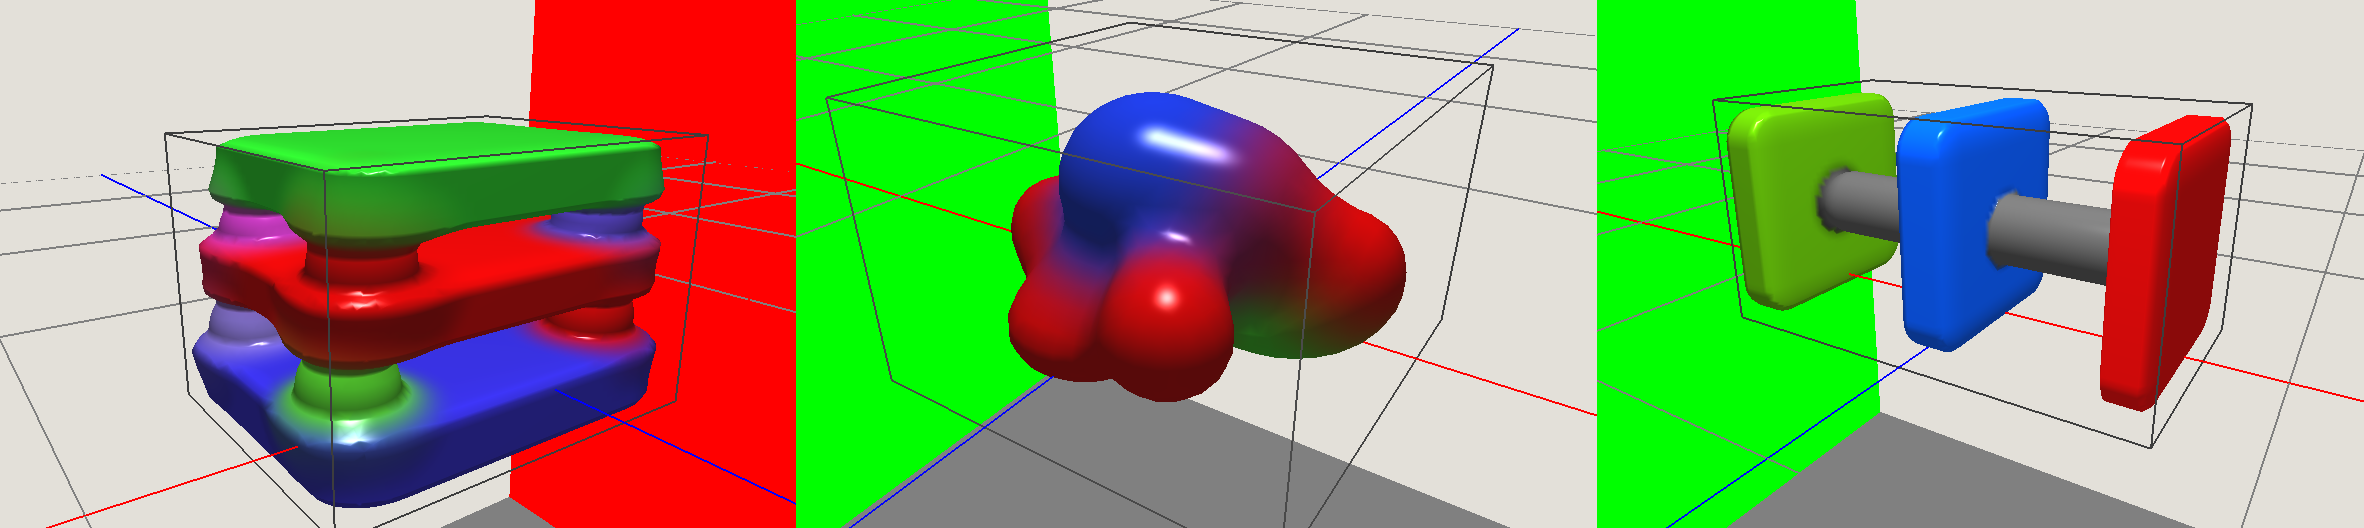
\includegraphics[width=1.0\linewidth]{figures/gpupoly/combined_models.png}
  \caption{\label{fig:combinedmodels}
  {Sample models for testing our GPU polygonization method. From left to right: Cake, tumor and 3slabs.}
}
\end{figure}

When using stacks, the register spilling phenomenon mentioned previously degrades the performance due to the higher cost of accessing 
the shared memory. Conditional push and pops in the stack-based method also stalls the performance of the kernels.  

Faster field evaluations using the stackless algorithm also improved the performance of our root-finding method and the overall
polygonization time. In the following we review per kernel time break-time which provides a close look at hotspots (most time-consuming 
locations) in our implementation. 

%Tumor: Fields: 2, Edge: 1, EdgeBufferScan: 22, Vertex: 44, Cell: 1, FaceBufferScan: 18, Faces: 17, Total: 105
%Cake: Fields: 1, Edge: 1, EdgeBufferScan: 19, Vertex: 58, Cell: 2, FaceBufferScan: 17, Faces: 10, Total: 108
%3Slabs: Fields: 1, Edge: 1, EdgeBufferScan: 18, Vertex: 40, Cell: 1, FaceBufferScan: 17, Faces: 1, Total: 79

\begin{figure}[H]
  \centering
  % the following command controls the width of the embedded PS file
  % (relative to the width of the current column)
  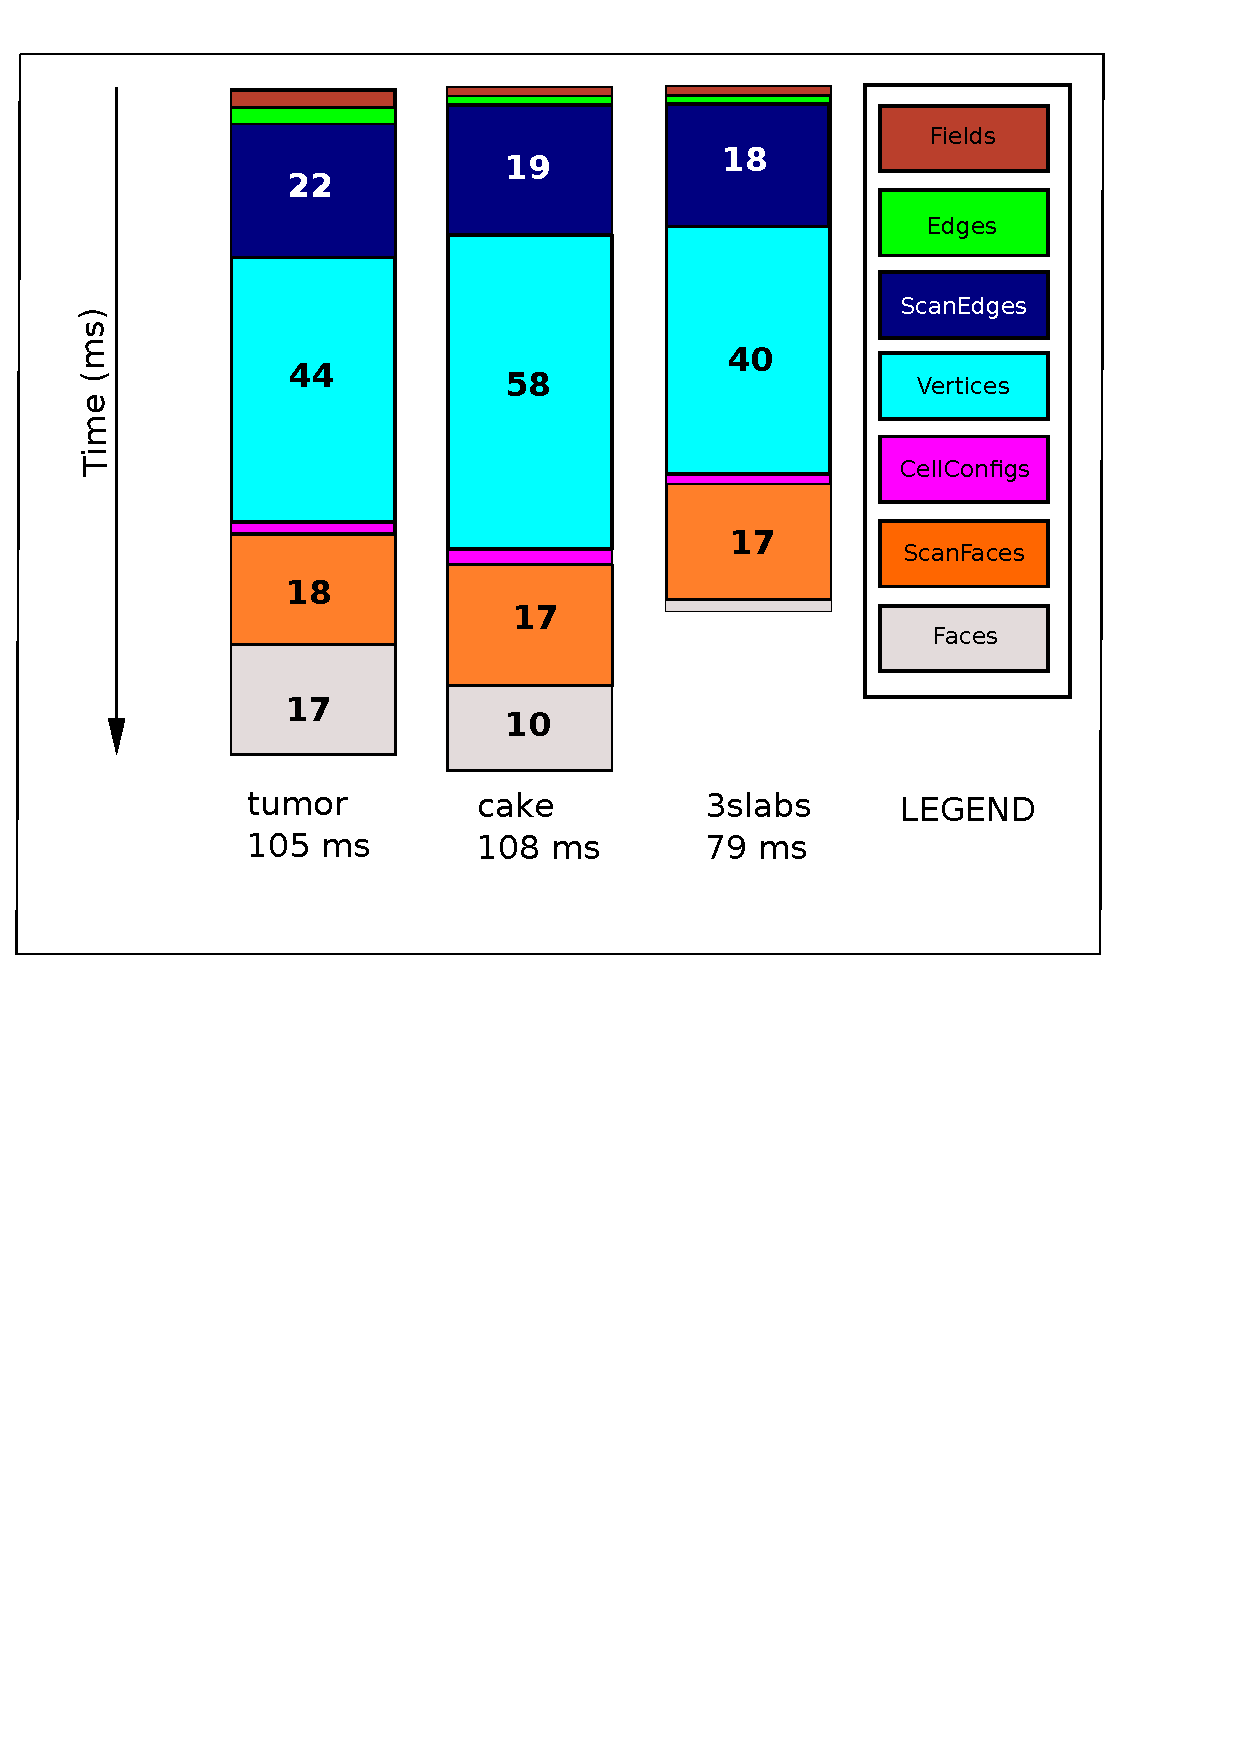
\includegraphics[width=0.8\linewidth]{figures/gpupoly/breakdownpoly.pdf}
  \caption{\label{fig:breakdownpoly}
  {Polygonization time breakdown in milliseconds for the three models shown in the previous section. Vertex processing is the most compute-intensive
  stage due to the Newthon-Raphson root finding method employed and the evaluation of colors and normals which require additional traversals.
  }
}
\end{figure}

As it can be seen computing vertices is still the most time-consuming stage due to the extra tree traversals required for high quality 
gradiant-based Newthon-Raphson root-finding method. Computing other attributes such as colors and normals would also need 1 and 4 
traversals respectively. The prefix-sum scan operator employed here uses multi-pass computing. The extra cost of kernel calls has
increased the cost of using these operators. Several optimizations can be performed to benefit the overall performance. By 
vectorizing all kernels the core SIMD units can be used more efficiently. 
In Nvidia and AMD GPUs the local memory is divided into memory banks. Each bank can only address one dataset at a time, so if a halfwarp (16 threads)
tries to load/store data from/to the same bank the access has to be serialized (this is called a bank conflict). 
For NVidia GT200 GPUs there are 16 banks and in Fermi card this number is 32. If each thread in a halfwarp accesses successive 32bit values
there are no bank conflicts. An exception from this rule are broadcasts: If all threads access the same address, the value is only read once and
broadcasted to all threads (e.g. For GT200 it has to be all threads in the halfwarp accessing the same address).

The prefix-sum scan operator can also be implemented in such a way that the memory-bank conflicts are completely avoided and the data-accesses
are performed in parallel.



















